% Chapter 1

\chapter{Introducción general} % Main chapter title

\label{Chapter1} % For referencing the chapter elsewhere, use \ref{Chapter1} 
\label{IntroGeneral}

%----------------------------------------------------------------------------------------

% Define some commands to keep the formatting separated from the content 
\newcommand{\keyword}[1]{\textbf{#1}}
\newcommand{\tabhead}[1]{\textbf{#1}}
\newcommand{\code}[1]{\texttt{#1}}
\newcommand{\file}[1]{\texttt{\bfseries#1}}
\newcommand{\option}[1]{\texttt{\itshape#1}}
\newcommand{\grados}{$^{\circ}$}

%----------------------------------------------------------------------------------------

%\section{Introducción}

%----------------------------------------------------------------------------------------
En este apartado se introducen los conceptos básicos sobre vehículos eléctricos, las tecnologías existentes y los objetivos propuestos para resolver las necesidades planteadas por el cliente.

\section{Vehículos eléctricos}

Un vehículo eléctrico es un vehículo propulsado por uno o más motores eléctricos. Este puede alimentarse a través de una fuente externa, baterías o paneles solares \citep{faiz1996air}. 
Los vehículos eléctricos han sido identificados como una tecnología clave para reducir las emisiones futuras y el consumo de energía en el sector de la movilidad \citep{helmers2012electric}.

\subsection{El tren motor}

El tren motor es el componente que caracteriza y distingue al vehículo eléctrico respecto a los vehículos a combustión. Este puede dividirse en cuatro partes principales: la batería, su cargador, 
el controlador del motor y el motor eléctrico (figura \ref{fig:vehículo_electrico}).
La batería se carga con electricidad cuando se conecta a la red eléctrica a través de un dispositivo de carga o durante el frenado a través de la recuperación. El 
controlador de motor suministra al motor eléctrico una potencia variable en función de la situación de la carga. El motor eléctrico convierte la energía eléctrica en energía mecánica que finalmente se traduce 
en el torque necesario para impulsar el vehículo \citep{larminie2012electric}.

\begin{figure}[h]
	\centering
	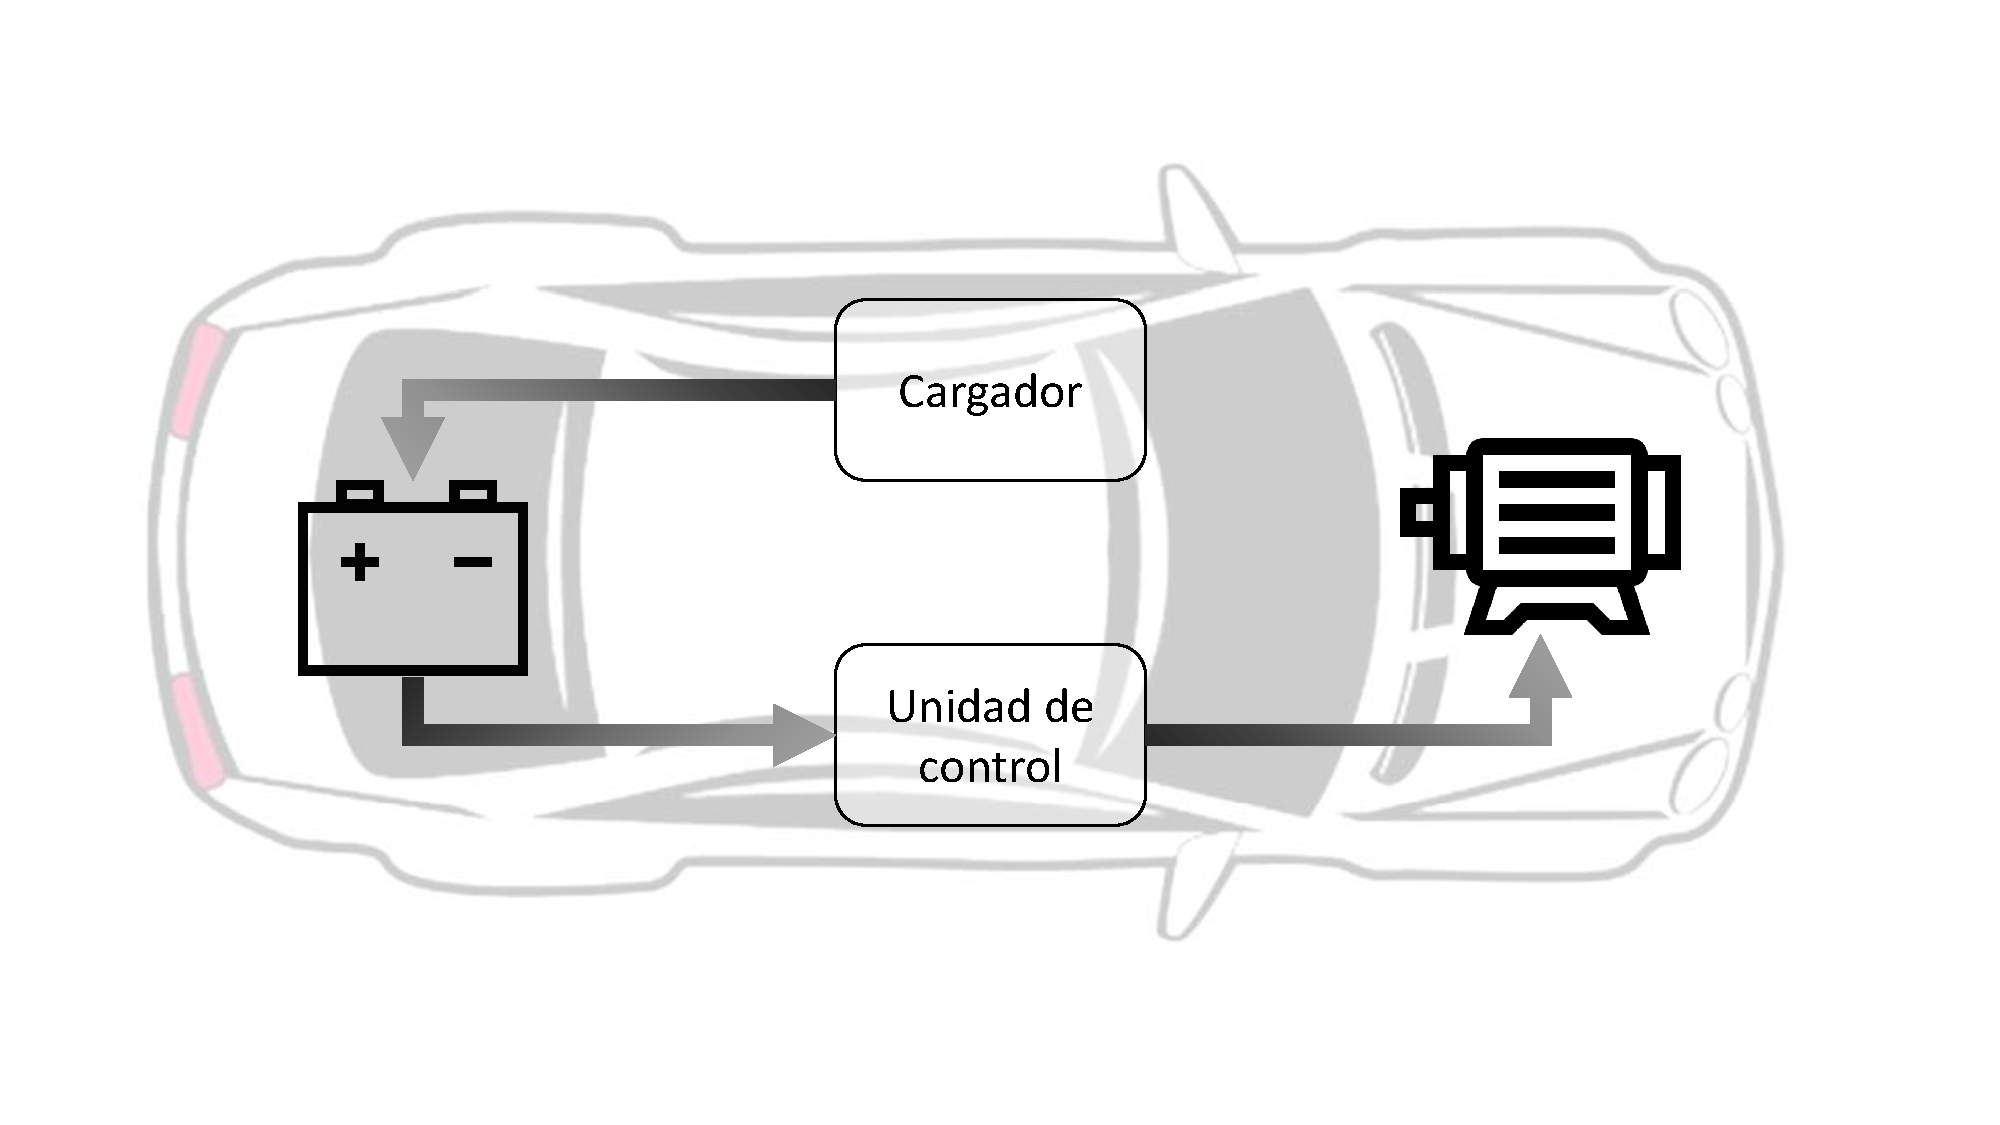
\includegraphics[width=\textwidth]{./Figures/VehiculoElectrico.pdf}
	\caption{Componentes importates de un vehículo eléctrico}
	\label{fig:vehículo_electrico}
\end{figure}

\subsubsection{Batería}
La batería es un componente que almacena la energía eléctrica necesaria para el funcionamiento del vehículo. Actualmente se utizan baterías de tipo Li-ion debido a la gran densidad de energía 
que estas pueden ofrecer. Hoy en día diferentes alternativas de baterías de Litio están disponibles y los precios decrecen continuamente \citep{helmers2012electric}.

\subsubsection{Cargador}
El cargador es el elemento que gestiona la inyección de corriente eléctrica desde la red a la batería. Además de inyectar corriente a la batería el cargador interactúa con 
la estación de carga para asgurar que el consumo del vehículo no supere el permitido por la instalación donde se conecta.

\subsubsection{Controlador}
El controlador es el encargado de suministrar la corriente eléctrica necesaria al motor eléctrico según la velocidad y potencia deseada por el usuario. 
Estos son dispositivos microcontrolados que interpretan señales (como la del acelerador) y mediante un inversor DC-DC o DC-AC controlan la potencia del motor.

\subsubsection{Motor}
El motor es el componente encargado de convertir la energía eléctrica en energía mecánica. Los motores eléctricos más modernos y eficientes están basados en imanes permanentes, 
pero los materiales para la construcción de estos motores (como el neodimio) son escasos. Existen alternativas sin imanes permanentes que son más económicos y muy utilizados en 
vehículos eléctricos \citep{helmers2012electric}.

\subsection{Ventajas de un vehículo eléctrico}

El vehículo eléctrico puro tiene una ventaja incomparable sobre los vehículos de combustión interna convencionales en términos de conservación de energía, emisiones de gases y garantía de la seguridad 
del suministro de petróleo. El hecho de que el vehículo eléctrico produzca cero emisiones es de gran interés para fabricantes y gobiernos \citep{karki2020status}.
Un ejemplo para dimensionar el impacto de esta tecnología es que la Unión Europea ya definió la prohibición de coches con motor de combustión interna a partir del año 2035 \citep{WEBSITE:1}.

%----------------------------------------------------------------------------------------

\section{Estado del atre}

CONSULTA: En mi trabajo desarrollé el firmware de una placa que pertenece al power train. La solución de Voltu tiene dos placas microcontroladas. Antes también tenía dos placas microcontroladas, pero una realizaba todas las tareas y la segunda solo gestionaba la comunicación usb.
Esto llevó a que la primera se encuentre saturada y esto limitaba el crecimiento del producto.
El nuevo diseño es un cambio interno en la configuración de la unidad de control. El que antes era el microcontrolador más chico se convierte en el microcontrolador más 
grande y se le asignan todas las tareas que no son exlusivas del control de potencia.
En resumen el desarrollo realizado es un firmware que cumple con las funcionalidades que 
antes hacia la placa de comunicaciones existente más funcionalidades trasladadas de la placa de control a la nueva placa de comunicaciones.
Hablar de características de los trenes motores como eficiencia, potencia, autonomía, tiempo de carga no me aporta información relevante para los cambios o aportes que tuvo mi desarrollo.
Mi desarrollo permitió que se le retirara carga a la placa de control y como consecuencia mejorar significativamente la estabilidad del sistema. Además se sentaron las bases para que el 
producto pueda escalar en el futuro facilmente desde el sistema actual.

¿Qué contenido se espera en el estado del arte que aporte al trabajo realizado?

En mente tenía mostrar una tabla comparando la distribución de resposabilidades de ambas placas en el sistema viejo para que se pueda entender más adelante como se redistribuyen las resposabilidades. ¿Es válido? ¿Es lo que se espera para esta sección? ¿Cómo puedo comparar esto con otros sitemas comerciales?

\section{Motivación}
Como se ha mencionado anteriormente existe una necesidad global emergente sobre el reemplazo de los vehículos de combustión interna por vehículos con cero emisiones. Los vehículos 
eléctricos aparecen como la alternativa más prometedora. Voltu Motors desarrolla trenes motores para vehículos eléctricos como principal producto de su compañía. Como una actualización a su producto
ha reemplazado el hardware para mejorar la estabilidad del sistema y poder proyectar nuevas características en función a lo demandado por los clientes.

Este cambio implica un firmware completamente nuevo que debe estar funcional dentro de los plazos comerciales de la empresa. El desafío de definir desde el inicio
un firmware que determinará la escalabilidad y estabilidad del nuevo sistema, y la oportunidad de ser parte de esta revolución tecnológica es la principal motivación para encarar este proyecto. 

\section{Objetivos y alcance}

El propósito de este proyecto es desarrollar el firmware de la nueva placa de comunicaciones. Este firmware debe cubrir las características de la versión anterior y además contemplar 
el manejo del sistema de administración de baterías, la interacción con la estación de carga y los periféricos.
La nueva versión también será la encargada de realizar el control de temperatura del sistema.

En el presente proyecto se diseñará, desarrollará e implementará el firmware de la placa de comunicaciones hasta que sea funcional para un vehículo que utilice una sola unidad de tren motor.
Esto incluye la implementación de las siguientes características:
\begin{itemize}
	\item Manejo de entradas y salidas digitales.
	\item Comunicación USB para la comunicación con el tablero.
	\item Comunicación con placa de control, transmisión de datos y recepción de datos.
	\item Gestión del estado del vehículo.
	\item Administración de la batería (definir cuando cargar y balancear las celdas).
	\item Control de temperatura del sistema.
\end{itemize}